% Preamble
\documentclass[a4paper, 12pt]{article}
\usepackage[margin=1in]{geometry} % Set margin
\usepackage{pdfpages} % Insert pdf pages
\usepackage{amssymb,amsmath,amsthm, amsfonts} % Math libraries

% Custom commands
\newcommand{\sub}[1]{\subsection{\underline{#1}}}
\newcommand{\subsub}[1]{\subsubsection{\underline{#1}}}
\newcommand{\?}{\stackrel{?}{=}}
\newcommand{\R}{\ensuremath{\mathbb{R}}}
\newcommand{\F}{\ensuremath{\mathbb{F}}}
\newcommand{\Onef}{\ensuremath{1_{\F}}}
\newcommand{\Zerof}{\ensuremath{0_{\F}}}
\newcommand{\eqbcuz}[1]{\text{~$\stackrel{(#1)}{=}$~}}
\newcommand{\eq}[1]{\begin{align*}#1\end{align*}}
\newcommand{\eqn}[1]{\begin{align}#1\end{align}}
\renewcommand{\qed}{$$\blacksquare$$}
\renewcommand{\b}[1]{\textbf{#1}}
\renewcommand{\because}[1]{~\b{(#1)}\\}
\renewcommand{\d}{\ensuremath{\Downarrow\\~}}
\newtheorem{lemma}{Lemma}

% Begin Document %
\begin{document}

% Title Page
\begin{titlepage}
    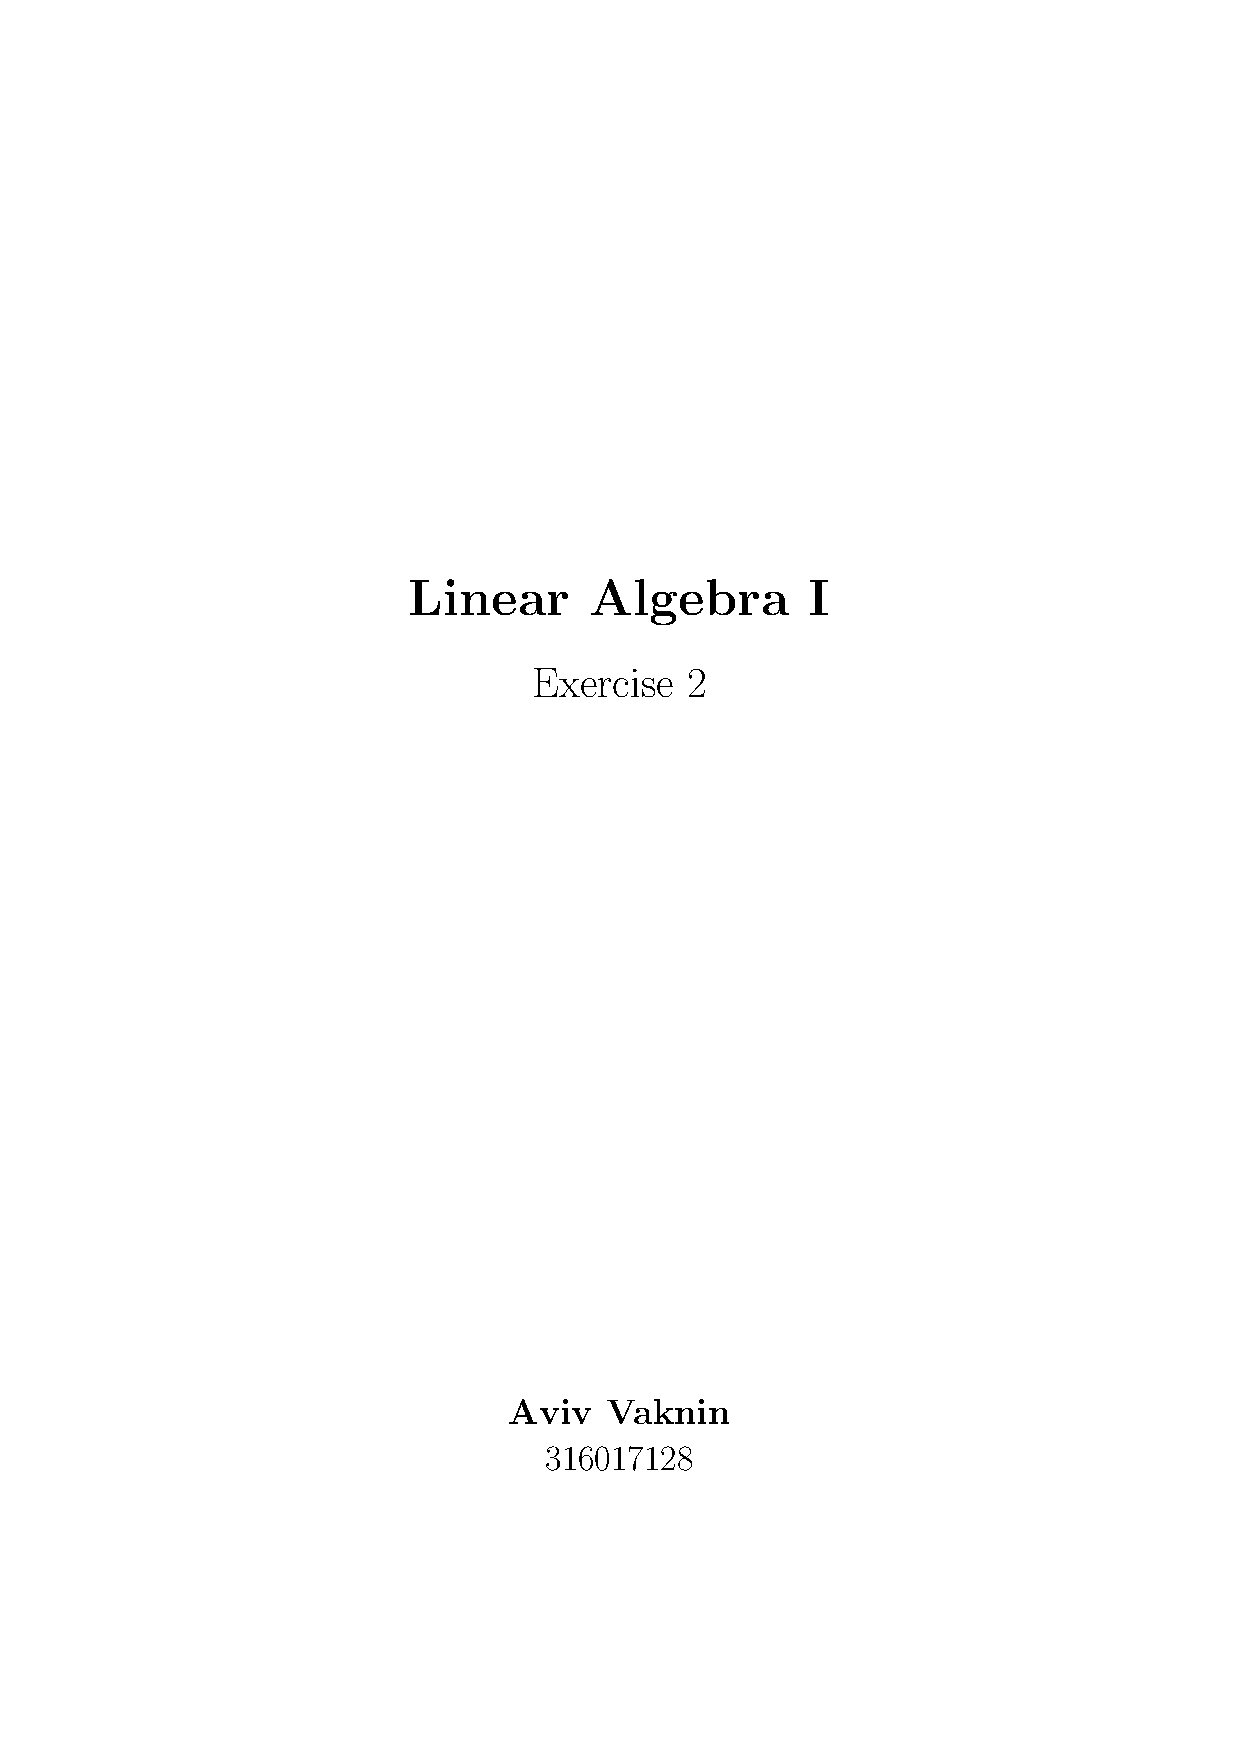
\includepdf{title.pdf}
\end{titlepage}

% 7
\setcounter{section}{6}
\section{Find the solution set for: $$X+Y-Z=-1$$ $$X-Y-Z=-1$$}
First, let's isolate $X$:
$$ X=Z-Y-1 $$
$$ X=Z+Y-1 $$
From the above, we can conclude that $Y=0$.
If we change one of the original equations, we'll get: $$ X=Z-1 $$
Therefore, the solution set for $X,Y,Z$ is:
$$
S = \Bigg{\{}
    \bordermatrix {
    &        \cr
    & z-1    \cr
    & y    \cr
    & z    \cr
    }
:
y, z \in {\R}
\Bigg{\}}
$$
\qed

% 8
\section{Show that the inverse of the inheritance rule is not true.}
The equations system:
$$ x^1 + x^2 = 1 $$
$$ x^2 - x^3 = 3 $$

We can generate the equation $L$, which is a linear form of the mentioned two equations,
by multiplying the first equation by $3$, and the second one by $(-1).$
$$ L: 3x^1 + 2x^2 + x^3 = 0 $$

As we can easily see, the following solution to $L$ is not a solution to the equations system:
$$ x^1=0 $$ $$ x^2=0 $$ $$ x^3=0 $$
\qed\pagebreak

% 10
\setcounter{section}{9}
\section{Are the two equation systems equivalent? if yes, write every equation as a linear form of the other system.}
\sub{Showing the systems are equivalent}
\subsub{Right-hand side system}
First, let's find the solutions set of the right-hand side system.\\
We can easily see from the first equation that $X^1=X^3$, in addition, let's declare $t^1=X^3$.\\
Now, from the second equation, we get: $$ X^2 = -3t^1 $$
This leads us to the following solutions set for the right-hand side system:
$$
S = \Bigg{\{}
    \bordermatrix {
    &        \cr
    & t^1    \cr
    & -3t^1    \cr
    & t^1    \cr
    }
:
t^1 \in {\R}
\Bigg{\}}
$$

\subsub{Left-hand side system}
Let's find the linear form of $L_2-2L_3$: $$ X^2+3x^3 = 0 $$
Which leads us to: $$ X^2 = -3x^3 $$
In addition, we'll mark $X^3$ as $t^1$, i.e.: $$X^2 = -3t^1$$
Now, we'll find the linear form of $L_2-2L_1$: $$ 3x^1-3t^1 = 0 $$
Which leads to:
$$ 3x^1 = 3t^1 $$
$$ x^1 = t^1 $$
This leads us to the following solutions set for the left-hand side system:
$$
S = \Bigg{\{}
    \bordermatrix {
    &        \cr
    & t^1    \cr
    & -3t^1    \cr
    & t^1    \cr
    }
:
t^1 \in {\R}
\Bigg{\}}
$$
As we can see, the two systems have identical solution sets, thus, they're equivalent.
\pagebreak

\sub{Write as a linear form of the other system}
\subsub{Left-hand side system as a linear form of the other system}
$$ -X^1 + X^2 + 4X^3 = 0 $$
If we multiply the first and second equations by $(-1)$ and $(1)$, respectively, we'll receive the intended equation.
$$ X^1 + 3X^2 + 8X^3 = 0 $$
If we multiply the first and second equations by $(1)$ and $(3)$, respectively, we'll receive the intended equation.
$$ \frac{1}{2}X^1 + X^2 + \frac{5}{2}X^3 = 0 $$
If we multiply the first and second equations by $(\frac{1}{2})$ and $(1)$, respectively, we'll receive the intended equation.

\subsub{Right-hand side system as a linear form of the other system}
$$ X^1 - X^3 = 0 $$
If we multiply the first, second and third equations by $(-\frac{3}{4})$, $(\frac{1}{4})$ and $(0)$, respectively, we'll receive the intended equation.
$$ X^2 + 3X^3 = 0 $$
If we multiply the first, second and third equations by $(\frac{1}{4})$, $(\frac{1}{4})$ and $(0)$, respectively, we'll receive the intended equation.
\qed\pagebreak

% 13
\setcounter{section}{12}
\section{Does a homogenous system of $m$ linear equations with $n$ variables with a single solution exist?}
\sub{$n=3,~m=4$}
It exists, here's an example of such a system:
$$ x+y+z=0 $$
$$ 2x+2y+2z=0 $$
$$ 3x+3y+3z=0 $$
$$ 4x+4y+4z=0 $$
\sub{$n=4,~m=3$}
It doesn't exist.

% 16
\setcounter{section}{15}
\section{Write the equation system that the given matrix, is its coefficients matrix}
$$ 0x^1+0x^2+x^3+4x^4+3x^5=0 $$
$$ 2x^1+4x^2+2x^3+6x^4+7x^5=0 $$
$$ 3x^1+6x^2+2x^3+5x^4+8x^5=0 $$

% 18
\setcounter{section}{17}
\section{Can $A$ and $B$ be row-equivalent? explain why.}
There aren't any elementary row operations that can be applied to $A$ or $B$, so that they'll be row-equivalent.\\
That is because their columns and rows count are different.\\
In other words, there does not exist a sequence $e_1,e_2...e_s$ such that:
$$ A = e_s(e_{s-1}(...e_1(B))) $$
\pagebreak

% 19
\section{}
\sub{What are the inverse operations to $e_{1}^{-1},e_{2}^{-1},e_{3}^{-1}$?}
\subsub{$e_{1}^{-1}$:}
The inverse is simply: $$ e_{1}^{-1} = A^1\cdot (-2)^{-1} $$
Such that: $$ e_{1}^{-1}(e_{1}(A^1)) = A^1 $$

\subsub{$e_{2}^{-1}$:}
The inverse is simply itself: $$ e_{2}^{-1} = e_{2} $$
Such that: $$ e_{2}(e_{2}(A)) = A $$

\subsub{$e_{3}^{-1}$:}
Because $e_{3}$ is: $$ e_{3} = A^3+3\cdot{A^1} $$
The inverse is: $$ e_{3}^{-1} = A^3-3\cdot{A^1} $$

\sub{Execute $e_{1}^{-1},e_{2}^{-1},e_{3}^{-1}$ on the matrix}
\begin{align*}
    e_1(A) &=
    \begin{bmatrix}
        4&2&-2&6\\
        1&-2&0&1\\
        0&0&2&1
    \end{bmatrix}
    \\\\e_2(e_1(A)) &=
    \begin{bmatrix}
        1&-2&0&1\\
        4&2&-2&6\\
        0&0&2&1
    \end{bmatrix}
    \\\\e_3(e_2(e_1(A))) &=
    \begin{bmatrix}
        1&-2&0&1\\
        4&2&-2&6\\
        3&-6&2&4
    \end{bmatrix}
\end{align*}
\pagebreak

% 23
\setcounter{section}{22}
\section{$B$ is row-equivalent to $A$, and $C$ is row-equivalent to $B$.\\Prove $C$ is row-equivalent to $A$.}
First, let's prove that every row is row-equivalent to itself.\\
Let's suppose that $e$ is an elementary operation that multiplies the first row by $1$.\\
Because of that, we can see that $A$ is row-equivalent to $A$:
\begin{align}
    A = e(A)
\end{align}
That proves that every matrix is row-equivalent to itself.\\
It is given that $B$ is row-equivalent to $A$, therefore by definition,
there exists a series of elementary operations $e_{1},e_{2}...e_{j}$ such that:
\eqn{B = e_{j}(e_{j-1}(...e_{1}(A)))}
Since every operation $e$ has an inverse operation $e^{-1}$, using $(2)$ we can see that:
\eq{e_{j}^{-1}(B) = e_{j}^{-1}(e_{j}(e_{j-1}(...e_{1}(A)))) = e_{j-1}(...e_{1}(A))}
We can now use induction to see that if we keep performing these operations, we'll eventually arrive at $A$.\\
Therefore, since we've placed operations on $B$ and from that arrived to $A$,\\
we've shown that if $g$ is row-equivalent to $h$, $h$ is row-equivalent to $g$.\\
Therefore, that implies that both $A$ and $C$ are row-equivalent to $B$, and therefore, they're row-equivalent as well.
\qed\pagebreak

% 24
\section{Prove:}
\eq{
    ad-bc\neq{0} \implies
    \begin{bmatrix}
        a&b\\
        c&d
    \end{bmatrix}
    \iff
    \begin{bmatrix}
        1&0\\
        0&1
    \end{bmatrix}
}
Let's divide it to cases.
\sub{$a=0$:}
Since $ad=0$, and $ad\neq{bc}$, we can assume that $bc\neq{0}$, which results in the following matrix, because $b,c$ are scalars,
and scalars can be changed to $1$ by performing elementary row operations on them.
\eq{A=\begin{bmatrix}
    0&1\\
    1&d
\end{bmatrix}}
We can now divide it into even deeper cases:
\subsub{$d=0$:}
If that is the case, the matrix is row equivalent (or even identical) to what we were trying to prove.
\subsub{$d\neq{0}$:}
Because d is just another scalar that is not $0$, we can perform some row operations (such as deducting $A^1$ from $A^2$) and make it $0$, for example:
\eq{
    \begin{bmatrix}
        0&1\\
        1&d
    \end{bmatrix}
    \longrightarrow(A^2-A^1)\longrightarrow
    \begin{bmatrix}
        0&1\\
        1&0
    \end{bmatrix}
}
\sub{$a\neq{0}$:}
\eq{A=\begin{bmatrix}
    a&b\\
    c&d
\end{bmatrix}}
Let's deduct $-\frac{a}{c}A^2$ from $A^1$, and we'll receive:
\eq{\begin{bmatrix}
    0&\frac{bc-ad}{c}\\
    c&d
\end{bmatrix}}
If we now deduct $-\frac{dc}{bc-ad}A^1$ from $A^2$, we'll get:
\eq{\begin{bmatrix}
    0&\frac{bc-ad}{c}\\
    c&0
\end{bmatrix}}
And from here, we can manipulate the two other scalars using elementary row operations to equal $1$, as requested.
\qed


% End Document %
\end{document}